\chapter{Experiments and Results}\label{exres}
In this chapter, the entire experimental process is presented, from the acquisition of the ground truth dataset (see section \ref{gt}), to the implementation, training and prediction phases of \modelnameshort\ (see section \ref{impdet}), and finally to the results evaluation and analysis (see section \ref{expres}).

\section{Ground Truth}\label{gt}
Our ground truth dataset consists of aerial images and buildings' coordinates, which are used as inputs and labels respectively when training. In this project, all of the aerial images are collected from Google Static Maps API and all of the latitude and longitude coordinates of the polygon vertices of buildings are collected from OpenStreetMap. For details of the two APIs mentioned above, please refer to subsections \ref{apimap} and \ref{apiosm}.

As mentioned in section \ref{modmer}, the training phase of our model \modelnameshort\ requires two different kinds of ground truth dataset, areas with multiple bounding boxes for FPN and buildings with geometrical shapes for PolygonRNN, both of which are illustrated in subsection \ref{arebui}.

Since the whole dataset is collected from two different sources, the problem of inconsistency may exist. Subsection \ref{proble} describes details of the problems in the ground truth dataset, and subsection \ref{adjust} proposes a feasible solution to adjust the shift between buildings' images and polygons.

\subsection{Google Static Maps API}\label{apimap}

Google Static Maps API\footnote{\lstinline{https://developers.google.com/maps/documentation/static-maps/}} provides an interface that implements maps as high-resolution images. Users can download customized map based on URL with different parameters, which is sent through a standard HTTPS request.

The parameters in URL includes the map type (satellite, roadmap, etc.), latitude and longitude coordinates of the image center, the resolution of the image, the zoom level, and the scale. For the usage of the Google Static Maps API, please refer to section \ref{app:apimap} in appendices. Figure \ref{fig:egsatellite} and \ref{fig:egroadmap} shows two types of images can be obtained by Google Static Maps API.

\begin{figure}[!h]
	\centering
	\subbottom[satellite image\label{fig:egsatellite}]
		{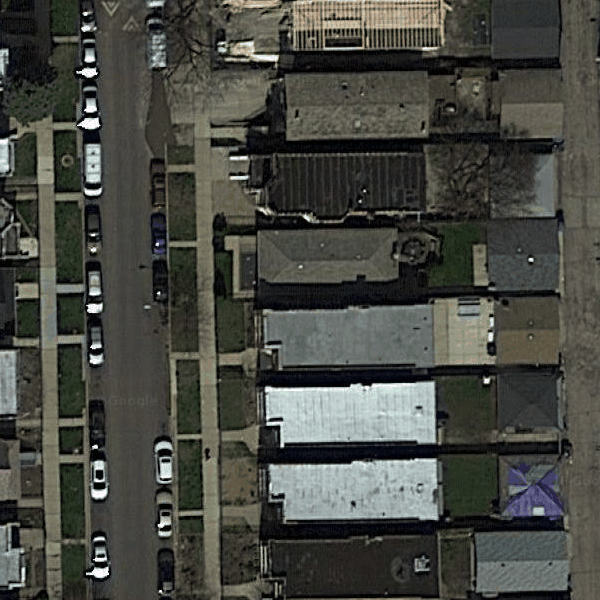
\includegraphics[width=0.328\textwidth]{4-00-0.png}}
	\subbottom[roadmap image\label{fig:egroadmap}]
		{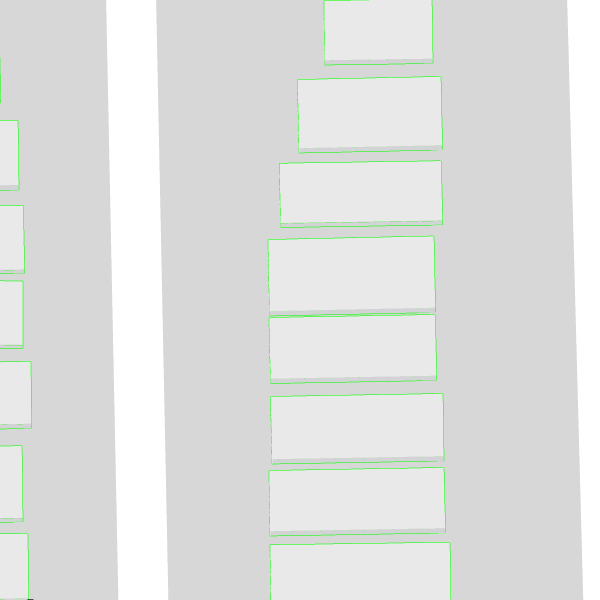
\includegraphics[width=0.328\textwidth]{4-00-1.png}}
	\subbottom[hybrid image\label{fig:eghybrid}]
		{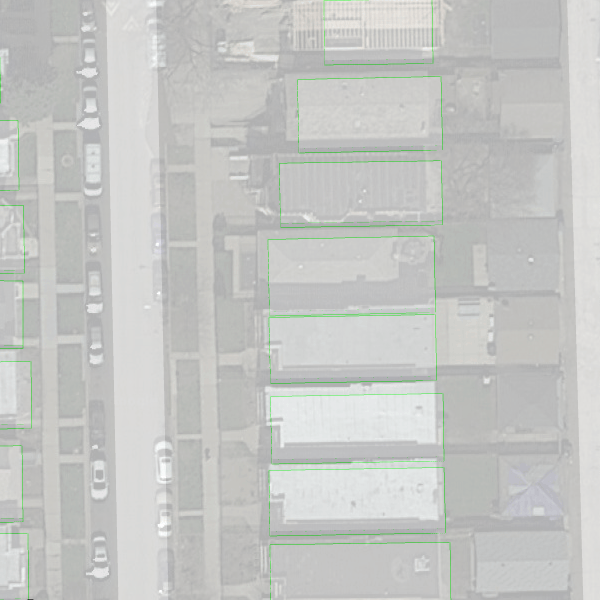
\includegraphics[width=0.328\textwidth]{4-00-2.png}}
    \caption{Example images downloaded through Google Static Maps API. (a) and (b) are obtained directly by the API, with 41.9399708 degrees north latitude, 87.7380649 degrees west longitude of the center (located in Chicago), both width and height 600 pixels, zoom level 20 and scale 1, but different in map types. (c) is obtained by overlaying (a) with (b), with 75\% opacity. It can be clearly seen that the two images cannot match very well.}
	\label{fig:egapimap}
\end{figure}

We would have liked to obtain buildings' coordinates from Google Static Maps API as well, but we find that the API does not provide such information directly. Instead, it gives the styled roadmap images like figure \ref{fig:egroadmap}, where querying coordinates requires further corner detection but the boundaries may be still inaccurate (see figure \ref{fig:eghybrid} for example). Thus, this thesis project, only satellite images from Google Static Maps API are used.

\subsection{OpenStreetMap}\label{apiosm}
OpenStreetMap\setcounter{footnote}{0}\footnote{\lstinline{https://www.openstreetmap.org/}} provides an interface that implements a map as a XML format \lstinline{.osm} file. The file contains all the information which can be used to recover the map. When the map's bounding box is given, users can retrieve the latitude and longitude coordinates of the buildings' vertices and roads' central lines within the map. For the usage of OpenStreetMap and the format of the \lstinline{.osm} file, please refer to section \ref{app:apiosm} in appendices.

The coordinates obtained by the API is the original latitude and longitude coordinates of the buildings' vertices, which cannot be directly used for training. We need to convert them to relative pixel coordinates with regards to an given satellite image.

As a matter of fact, every fixed point on the earth can correspond to a unique pixel on the map at a specific zoom level. This projection process can be regarded as a function. Since we have already known the relative pixel coordinates of the image center (half width and half height), the projection for an arbitrary point with given latitude and longitude coordinates can be therefore computed. This process can be described as
\begin{equation}
	(c_x, c_y) = (\frac{w}{2}, \frac{h}{2}) = f(c_{\text{lon}}, c_{\text{lat}}, z) + (\Delta_x, \Delta_y),
\end{equation}
\begin{equation}
	(p_x, p_y) = f(p_{\text{lon}}, p_{\text{lat}}, z) + (\Delta_x, \Delta_y),
\end{equation}
where $f$ is the function that projects latitude and longitude coordinates to global pixel coordinates (see \ref{app:projec} in appendices for more details), $c$ is the image center, $p$ is an arbitrary point, the subscripts $x$, $y$, $\text{lon}$, $\text{lat}$ mean the relative pixel and longitude and latitude coordinates respectively, $z$ is the zoom level, $\Delta$ is the translation constant from the global to the relative pixel coordinate system. Thus, we have
\begin{equation}
	(p_x, p_y) = f(p_{\text{lon}}, p_{\text{lat}}, z) - f(c_{\text{lon}}, c_{\text{lat}}, z) + (\frac{w}{2}, \frac{h}{2}),
\end{equation}
for any arbitrary point $p$.

In addition, we keep the order of a polygon to be anticlockwise when training. However, the orders of coordinates of polygon vertices obtained from OpenStreetMap are not fixed. Thus, the reverse operation for those polygon with clockwise order is required. Please refer to section \ref{app:revpoly} in appendices for more details.

\subsection{Areas and Buildings}\label{arebui}

As mentioned in section \ref{modmer}, \modelnameshort\ is formed by FPN and PolygonRNN. However, the training phase of these two models requires two different kinds of ground truth dataset.

\paragraph{Areas for FPN}
In subsection \ref{modfpn} we have shown that FPN aims at finding rectangular RoIs. Thus, training FPN generally requires a relatively large image with several objects in it. When considering our problem, an example of the ground truth can be an area of a city with several bounding boxes. Each box contains a single building, regardless of its tight polygon outline. Figure \ref{fig:egareafpn} gives an example area for training FPN and its visualized ground truth label.

\begin{figure}[!h]
	\centering
	\subbottom[example area\label{fig:egarea}]
		{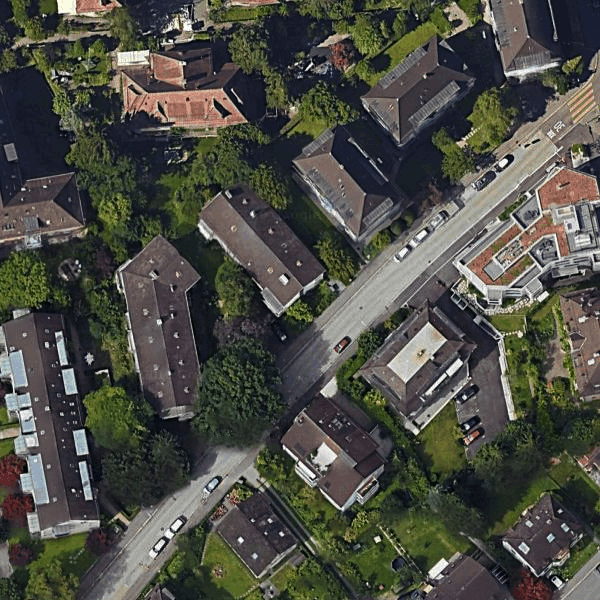
\includegraphics[width=\figfig\textwidth]{4-01-0.png}}
	\subbottom[example area with bounding boxes\label{fig:egareabox}]
		{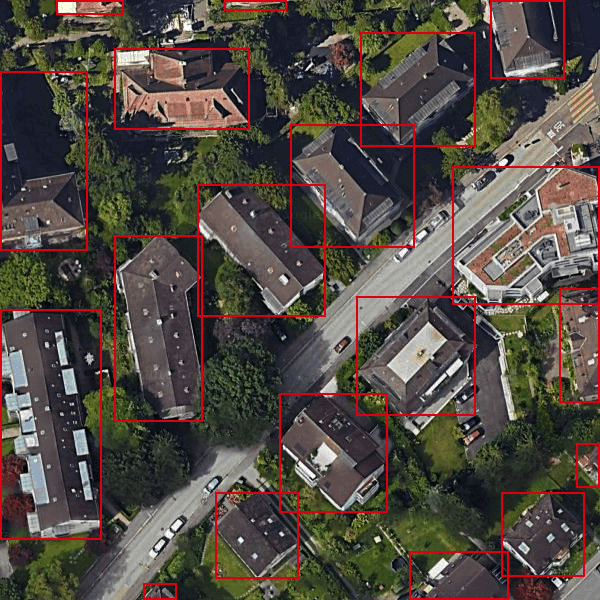
\includegraphics[width=\figfig\textwidth]{4-01-1.png}}
    \caption{An example area in Zurich for training FPN. (a) is the original satellite image obtained by Google Static Maps API. (b) is (a) covered by multiple bounding boxes of buildings, which is visualized based on the ground truth.}
	\label{fig:egareafpn}
\end{figure}

\paragraph{Buildings for PolygonRNN}
In section \ref{modpoly} we have mentioned that PolygonRNN can only deal with images with single object, meaning that the bounding box of the object should be first given. Thus, training PolygonRNN generally requires a relatively small image with single object, as well as the information of its polygon outline. When it comes to our problem, an example of the ground truth can be a building with some padding and the pixel coordinates of building's vertices. Figure \ref{fig:egbui} gives example buildings for training PolygonRNN and its visualized ground truth label.

\begin{figure}[!h]
	\centering
	\subbottom[\label{fig:egbui0}]
		{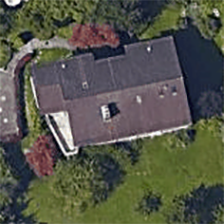
\includegraphics[width=0.243\textwidth]{4-02-0.png}}
	\subbottom[\label{fig:egbui1}]
		{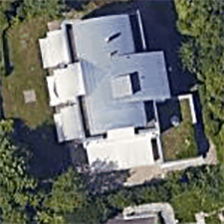
\includegraphics[width=0.243\textwidth]{4-02-1.png}}
	\subbottom[\label{fig:egbui2}]
		{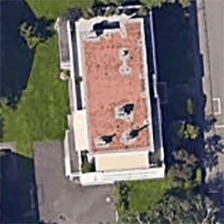
\includegraphics[width=0.243\textwidth]{4-02-2.png}}
	\subbottom[\label{fig:egbui3}]
		{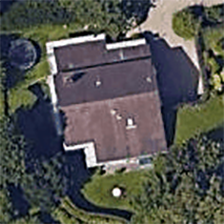
\includegraphics[width=0.243\textwidth]{4-02-3.png}}
	\subbottom[\label{fig:egbui4}]
		{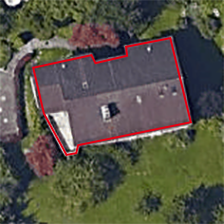
\includegraphics[width=0.243\textwidth]{4-02-4.png}}
	\subbottom[\label{fig:egbui5}]
		{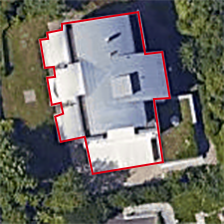
\includegraphics[width=0.243\textwidth]{4-02-5.png}}
	\subbottom[\label{fig:egbui6}]
		{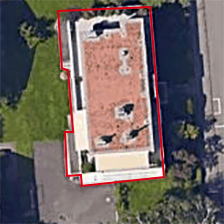
\includegraphics[width=0.243\textwidth]{4-02-6.png}}
	\subbottom[\label{fig:egbui7}]
		{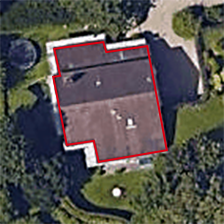
\includegraphics[width=0.243\textwidth]{4-02-7.png}}
    \caption{Example buildings in Zurich for training PolygonRNN. (a)-(d) are the original satellite images obtained by Google Static Maps API. (e)-(g) are (a)-(d) covered by the corresponding polygons' edges, which are visualized based on the ground truth.}
	\label{fig:egbui}
\end{figure}

\subsection{Problems}\label{proble}

Recall that the aerial images and polygons' coordinates are collected from two different sources, the problem of inconsistency may exist. That is to say, the polygon and the actual building we see in the image may not match well in some cases. This inconsistency is mainly reflected in the following aspects.
\begin{figure}[!h]
	\centering
	\subbottom[general shift\label{fig:egshi0}]
		{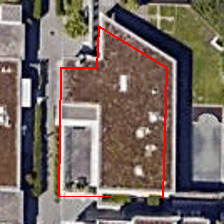
\includegraphics[width=0.243\textwidth]{4-03-0.png}}
	\subbottom[general shift\label{fig:egshi1}]
		{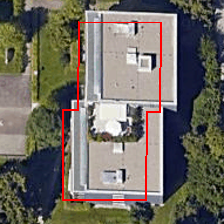
\includegraphics[width=0.243\textwidth]{4-03-1.png}}
	\subbottom[size too small\label{fig:egshi2}]
		{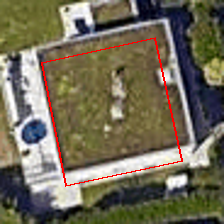
\includegraphics[width=0.243\textwidth]{4-03-2.png}}
	\subbottom[shape too rough\label{fig:egshi3}]
		{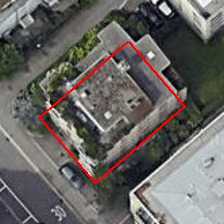
\includegraphics[width=0.243\textwidth]{4-03-3.png}}
	\subbottom[angle issue\label{fig:egshi4}]
		{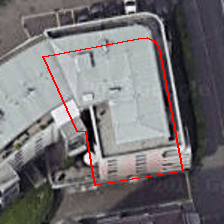
\includegraphics[width=0.243\textwidth]{4-03-4.png}}
	\subbottom[angle issue\label{fig:egshi5}]
		{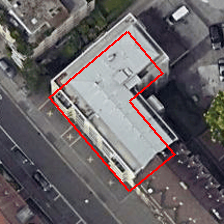
\includegraphics[width=0.243\textwidth]{4-03-5.png}}
	\subbottom[adjacent building\label{fig:egshi6}]
		{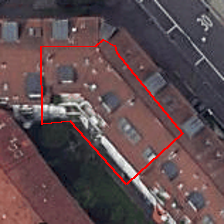
\includegraphics[width=0.243\textwidth]{4-03-6.png}}
	\subbottom[adjacent building\label{fig:egshi7}]
		{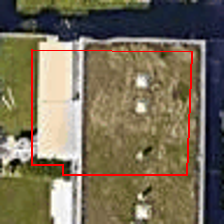
\includegraphics[width=0.243\textwidth]{4-03-7.png}}
    \caption{Problems existed in the ground truth dataset.}
	\label{fig:egshi}
\end{figure}
\begin{itemize}
	\item \textbf{General Shift}: Figure \ref{fig:egshi0} gives two typical shift examples in the dataset. The shift is generally within the range of 30 pixels, either up and down, or left and right.
	\item \textbf{Polygon Size and Shape}: Sometimes the polygon size and shape is different from the actual building size as well. This is typically because OpenStreetMap measures the bottom of the building and the aerial image is taken from the top. The roof of the house we see from the top can be different from the floor area. Figure \ref{fig:egshi1} shows a building with a smaller polygon and a building with a too rough outline.
	\item \textbf{Angle Issue}: Some tall buildings may suffer from the angle issue. This is because the aircraft that takes the image cannot always be vertically right above the building, so the side of those very high buildings would also be photographed. Figure \ref{fig:egshi2} gives two examples.
	\item \textbf{Adjacent Buildings}: Some adjacent buildings will be very close together, and some even share a common roof. Thus, from the aerial image, it is generally difficult to distinguish the boundaries between them. However, these buildings are separated in the dataset of OpenStreetMap. It means that where there are originally edges between buildings, it looks like there is no edge from the view of the aerial image. This kind of inaccuracy would have negative effect on the training phase. Figure \ref{fig:egshi3} and gives two examples.
\end{itemize}

\subsection{Adjustments}\label{adjust}
Problems such as too rough polygon shape, angle issue and adjacent buildings are unsolvable unless the data sources can correct themselves. What we can improve is to tackle the general shift and the polygon size problem and make the image-polygon pairs more matching. By observation, we can get to some conclusions for a matching image-polygon pair.
\begin{figure}[!h]
	\centering
	\subbottom[before adjustment\label{fig:egbfradj}]{
		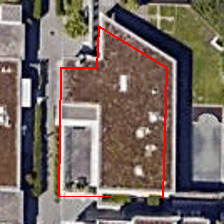
\includegraphics[width=\figfigfigfig\textwidth]{4-04-0.png}
		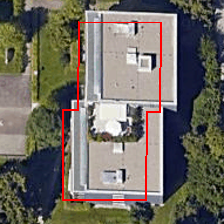
\includegraphics[width=\figfigfigfig\textwidth]{4-04-1.png}
		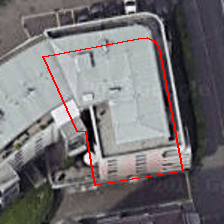
\includegraphics[width=\figfigfigfig\textwidth]{4-04-2.png}
		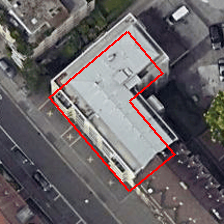
\includegraphics[width=\figfigfigfig\textwidth]{4-04-3.png}
	}
	\subbottom[after adjustment\label{fig:egaftadj}]{
		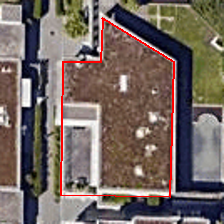
\includegraphics[width=\figfigfigfig\textwidth]{4-04-4.png}
		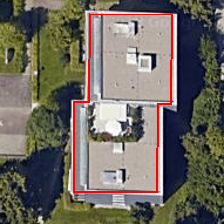
\includegraphics[width=\figfigfigfig\textwidth]{4-04-5.png}
		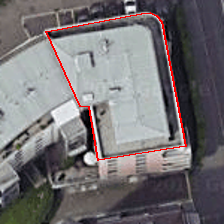
\includegraphics[width=\figfigfigfig\textwidth]{4-04-6.png}
		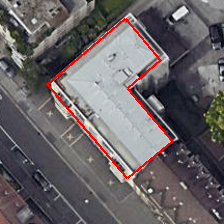
\includegraphics[width=\figfigfigfig\textwidth]{4-04-7.png}
	}
    \caption{Adjustment examples. (a) shows the polygons before adjustment, while (b) shows the polygons after adjustment.}
	\label{fig:egadj}
\end{figure}
\begin{itemize}
	\item \textbf{Color Variance}: The color variance of image pixels covered by polygon generally reaches the local minimum, because the roof of a building usually has only one color or several similar colors.
	\item \textbf{Edges}: The polygon edges generally lie within the output of the edge detection (e.g. Sobel, Canny) performed on the image.
	\item \textbf{Corners}: The polygon vertices can generally match the output of the corner detection (e.g. Harris, SIFT) performed on the image.
\end{itemize}

Based on these conclusions, we propose a brute force shift adjustment method. Briefly, we resize and translate the initial polygon within a certain range, and traverse all the cases to see where the minimum color variance, maximum edge and corner coverage are reached. The detailed algorithm, please refer to section \ref{app:shift} in appendices. Figure \ref{fig:egadj} illustrates some examples, which compare the polygons before and after the adjustment. Results show that this algorithm can well address the shift problem to some extent, which guarantees the correctness of the training set.

\section{Implementation Details}\label{impdet}

In this section, several implementation details are given in order to the replicate the model in the future if needed. Subsection \ref{datainfo} gives information and some notes of the dataset. Subsection \ref{config} gives the basic configuration of the model. Subsection \ref{trnphs} and \ref{prdphs} focus on the training and prediction phase respectively.

\subsection{Dataset Information}\label{datainfo}

The dataset consists of two cities, Zurich and Chicago, including most of the buildings in the range shown in table \ref{tab:bldrange}. In addition, aerial images are taken based on the information shown in table \ref{tab:arerange}.

\begin{table}[!h]
	\centering
	\caption[Sampling range of buildings in Zurich and Chicago]{Sampling range of buildings in Zurich and Chicago.}
	\label{tab:bldrange}
	\begin{tabular}{l|r|r}
	\hline
	\textbf{City} & Zurich & Chicago \\ \hline
	\textbf{East Boundary} & E $8.4092916^\circ$ & W $87.8039744^\circ$ \\
	\textbf{South Boundary} & N $47.2879518^\circ$ & N $41.8799477^\circ$ \\
	\textbf{West Boundary} & E $8.6729490^\circ$ & W $87.6721554^\circ$ \\
	\textbf{North Boundary} & N $47.4664863^\circ$ & N $41.97799394^\circ$ \\
	\hline
	\textbf{Number of Buildings} & 96,573 & 228,074 \\
	\textbf{Size of Training Set} & 86,915 & 205,266 \\
	\textbf{Size of Test Set} & 9,685 & 22,808 \\
	\hline
	\end{tabular}
\end{table}
\begin{table}[!h]
	\centering
	\caption[Sampling range of areas in Zurich and Chicago]{Sampling range of areas in Zurich and Chicago.}
	\label{tab:arerange}
	\begin{tabular}{l|r|r}
	\hline
	\textbf{City} & Zurich & Chicago \\ \hline
	\textbf{Center Longitude }& E $8.5468221^\circ$ & W $87.7380649^\circ$ \\
	\textbf{Center Latitude} & N $47.3768587^\circ$ & N $41.9289708^\circ$ \\
	\textbf{Step Longitude} & $4.023094^\circ\times10^{-4}$ & $4.469772^\circ\times10^{-4}$ \\
	\textbf{Step Latitude} & $2.724221^\circ\times10^{-4}$ & $3.324594^\circ\times10^{-4}$ \\
	\textbf{Horizontal Step Range} & $(-144, 144)$ & $(-144, 144)$ \\
	\textbf{Vertical Step Range} & $(-144, 144)$ & $(-144, 144)$ \\
	\textbf{Zoom Level} & 19 & 20 \\
	\textbf{Scale} & 1 & 1 \\
	\textbf{Image Size} & $(600, 600)$ & $(600, 600)$ \\
	\hline
	\textbf{Number of Areas} & 57,741 & 77,716 \\
	\textbf{Size of Training Set} & 51,966 & 69,944 \\
	\textbf{Size of Test Set} & 5,775 & 7,772 \\
	\hline
	\end{tabular}
\end{table}

There are some notes for buildings should be specified: (1) Buildings with more than 19 or less than 4 vertices are excluded; (2) All of the building images are squares but in different sizes, and include paddings; (3) As mentioned in subsection \ref{apiosm}, the order of all polygons are set to be anclockwise; (4) In each polygon, three consecutive vertices cannot be collinear. If so, the second vertex is removed.

There are some notes for areas should be specified: (1) Areas without any buildings are excluded; (2) There is an overlap between neighboring areas because each building is required to appear completely at least once within all areas. For example, in figure \ref{fig:egarea}, for the incomplete buildings locate near the image top edge, we can find them with complete shapes in its northern neighboring area.

\subsection{Model Configuration}\label{config}
Table \ref{tab:configpara} shows the parameters used to define the graph of model. The environment of implementation of our model is Python 3.6.1, with TensorFlow 1.6.0\setcounter{footnote}{0}\footnote{\lstinline{https://www.tensorflow.org/versions/r1.6/}}.
\begin{table}[!h]
	\centering
	\caption[Configuration parameters used to define the model graph]{Configuration  parameters used to define the model graph.}
	\label{tab:configpara}
	\begin{tabular}{l|r}
	\hline
	\textbf{Item} & \textbf{Value} \\
	\hline
	Area Image Resizing & $(256, 256)$ \\
	Building Image Resizing & $(224, 224)$ \\
	Resolution of Output Grid & $(28, 28)$ \\
	\hline
	RNN Max Sequence Length & 20 \\
	RNN Number of Layers & 3 \\
	ConvLSTM Number of Output Channels & $32, 16, 8$ \\
	\hline
	Feature Pyramid Number of Layers & 4 \\
	Anchor Scale & $16, 32, 64, 128$ \\
	Anchor Shape & $\frac{1}{2}$:2, $\frac{\sqrt{2}}{2}$:$\sqrt{2}$, 1:1, $\sqrt{2}$:$\frac{\sqrt{2}}{2}$, 2:$\frac{1}{2}$ \\
	Feature Shapes & 64$\times$64, 32$\times$32, 16$\times$16, 8$\times$8 \\
	Feature Stride & $4, 8, 16, 32$ \\
	Total Number of Anchors & 27,200 \\
	\hline
	\end{tabular}
\end{table}

\subsection{Training Phase}\label{trnphs}
During the training, buildings near the edges of aerial images are typically ignored since they are more likely to be incomplete. In this case, the polygon would be clipped by the edges, resulting in new vertices, which can be very hard to compute. Therefore, in this project, two different kinds of ground truth dataset are collected separately, which means that in a specific round of training, the building images come from the dataset instead of patches from aerial image. Training in this way can keep the batch size of buildings unchanged. Table \ref{tab:trnphs} shows the configuration parameters during the training phase of the model.

\begin{table}[!h]
	\centering
	\caption[Configuration parameters used in the training phase]{Configuration parameters used in the training phase.}
	\label{tab:trnphs}
	\begin{tabular}{l|r}
	\hline
	\textbf{Item} & \textbf{Value} \\
	\hline
	Optimizer & Adam \\
	Learning Rate & $1\times10^{-4}$ \\
	Area Batch Size & 4 \\
	Building Batch Size & 12 \\
	Number of Rounds & 25,000 \\
	\hline
	\end{tabular}
\end{table}

\subsection{Prediction Phase}\label{prdphs}
Recall subsection \ref{mulbboxreg}, an object bounding box may be regressed on multiple anchors, resulting in duplicate boxes. In order to get the best bounding box of an object, NMS (Non-Maximum Suppression) algorithm is adopted. NMS prunes away boxes that have high IoU overlap with previously selected boxes, thus the ``best" boxes can be remained. Figure \ref{fig:nms} shows an example of NMS algorithm. For more details about the algorithm, please refer to the paper \cite{softnms}, which includes both NMS and its improved version Soft-NMS.

\begin{figure}[!h]
	\centering
	\subbottom[before NMS\label{fig:bfrnms}]
		{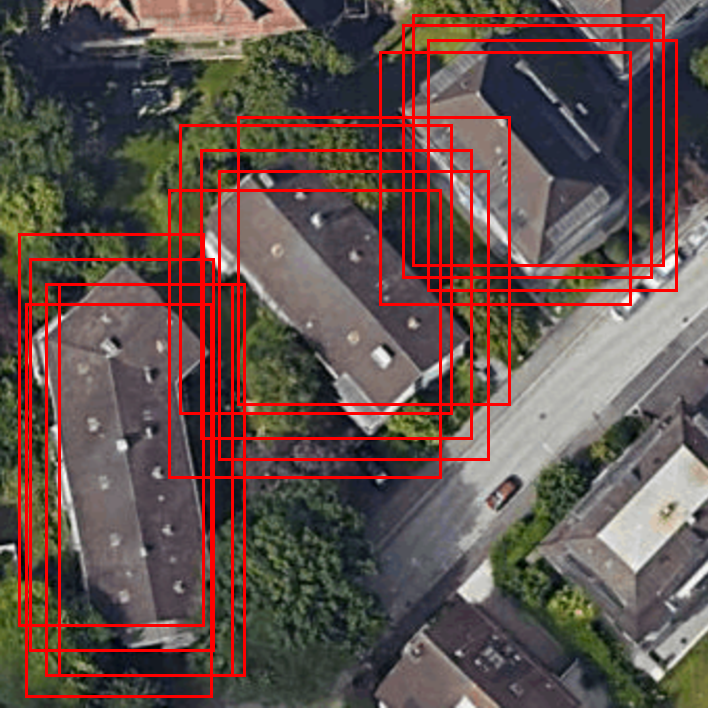
\includegraphics[width=\figfig\textwidth]{4-05-0.pdf}}
	\subbottom[after NMS\label{fig:aftnms}]
		{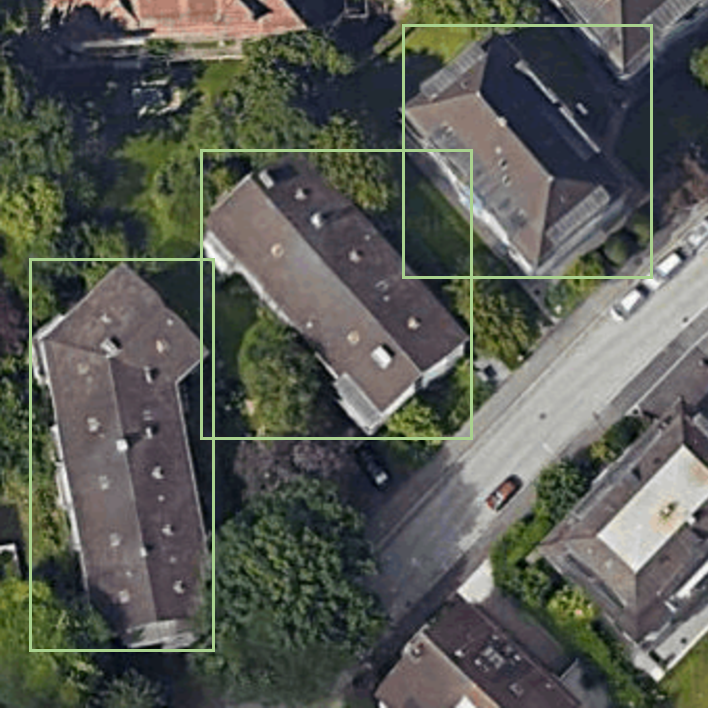
\includegraphics[width=\figfig\textwidth]{4-05-1.pdf}}
    \caption[Example of NMS algorithm]{Example of NMS algorithm.}
	\label{fig:nms}
\end{figure}
In practice, during the prediction, we first select a number of anchors with the highest (e.g. top 500) probability, and then remove anchors with probability lower than a threshold (e.g. 0.99). The selected anchors are then feed into NMS algorithm, which outputs the final RoIs. These RoIs are further taken as input of PolygonRNN to predict their geometrical shapes. Note that too small bounding boxes obtained by FPN are typically ignored and would not be used for polygon prediction. Table \ref{tab:prdphs} shows the configuration parameters during the prediction phase of the model.
\begin{table}[!h]
	\centering
	\caption[Configuration parameters used in the prediction phase]{Configuration parameters used in the prediction phase.}
	\label{tab:prdphs}
	\begin{tabular}{l|r}
	\hline
	\textbf{Item} & \textbf{Value} \\
	\hline
	Beam Width & 1 or 6 \\
	Top Number of Anchors & 500 \\
	Anchor Probability Threshold & 0.99 \\
	NMS Max Output Size & 40 \\
	NMS IoU Threshold & 0.15 \\
	Minimum Bounding Box Area & 16$\times$16 \\
	\hline
	\end{tabular}
\end{table}

\section{Experiment Results}\label{expres}
In this section, the experiment results are presented. We evaluate and analyze these results from different aspects. Subsection \ref{lossdec} focuses on loss decrease of both versions of the model. Subsection \ref{tmcsmp} records the time consumption in both training and prediction phases. Subsection \ref{evalmtc} uses kinds of metrics to evaluate the prediction results. Subsection \ref{predres} presents some prediction results of geometrical instance segmentation in aerial images, and makes comparison.

\subsection{Loss Decrease}\label{lossdec}
Figure \ref{fig:losdecch} and figure \ref{fig:losdeczh} show the loss decrease for all kinds of aspects in dataset of Chicago and Zurich, respectively. Note that in both figure, the loss of anchor classification, anchor regression, per-pixel mask prediction, and polygon vertices prediction are the 4 basic losses. The loss of FPN is calculated as the mean of anchor classification and regression losses, while the loss of PolygonRNN is calculated as the mean of mask and polygon prediction losses. The full loss is defined as the the mean of FPN loss and PolygonRNN loss. In the figures \ref{fig:losdecch} and \ref{fig:losdeczh}, the losses for two-step version are in shallow colors, while the losses for hybrid version are in deep colors.

We expect to draw some interesting conclusions from the comparison of the results of different cities or different models. From both figures we can conclude that the introduction of shared VGG-16 does not significantly accelerate the training phase of the network. The only change is that, the loss of RNN part (polygon vertices prediction) of PolygonRNN in the hybrid version falls earlier than the two-step version around the iteration 5,000. As for different cities, we find that the loss of Chicago decreases faster and finally becomes lower than the loss of Zurich. We consider that it is because most of the buildings in Chicago are vertically or horizontally aligned, thus it is easier for the machine to learn.

\begin{figure}[!h]
	\centering
	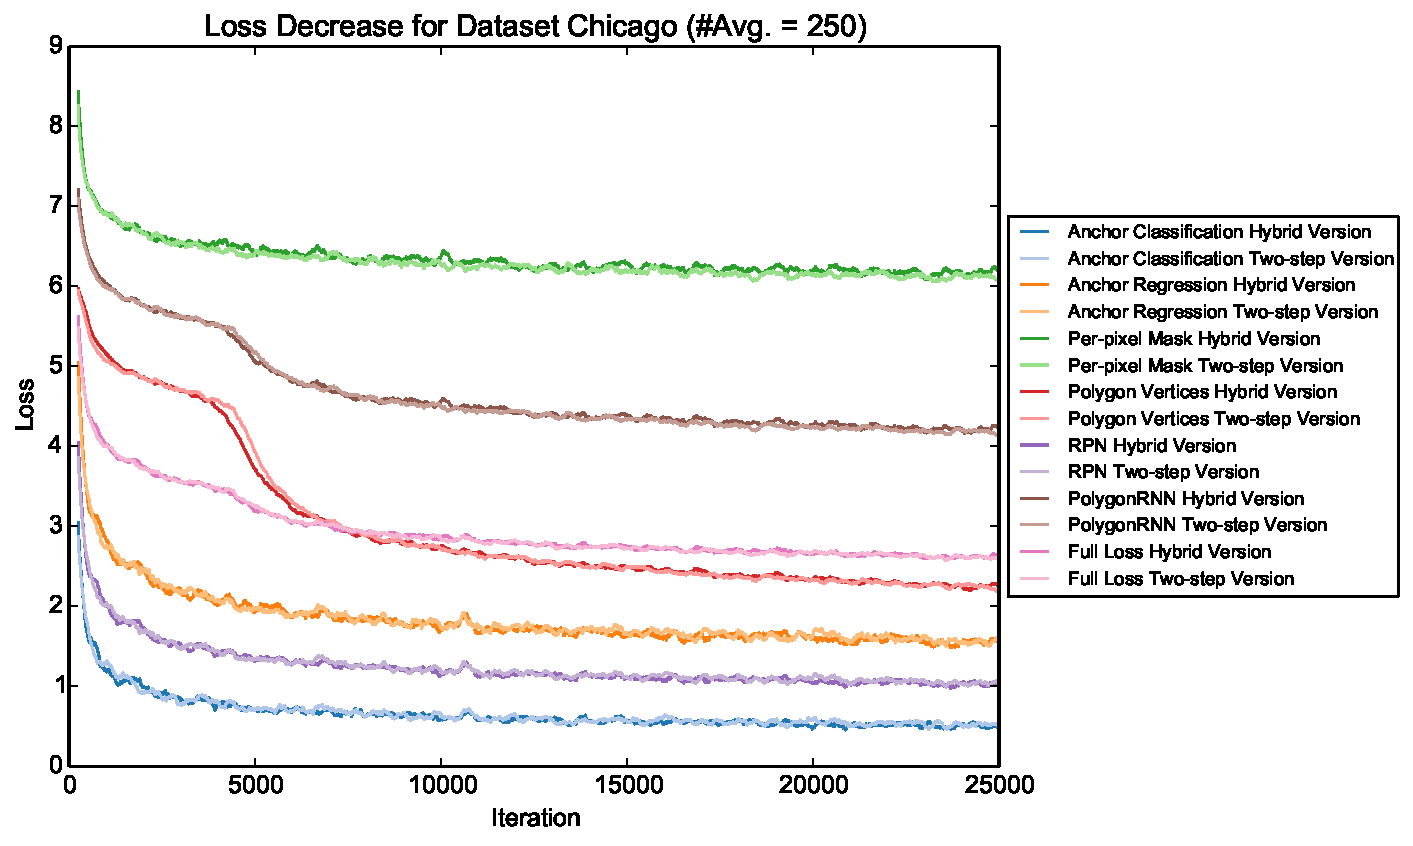
\includegraphics[width=\fig\textwidth]{4-06.pdf}
    \caption[Loss decrease of model in dataset Chicago]{Loss decrease of model in dataset Chicago.}
	\label{fig:losdecch}
\end{figure}
\begin{figure}[!h]
	\centering
	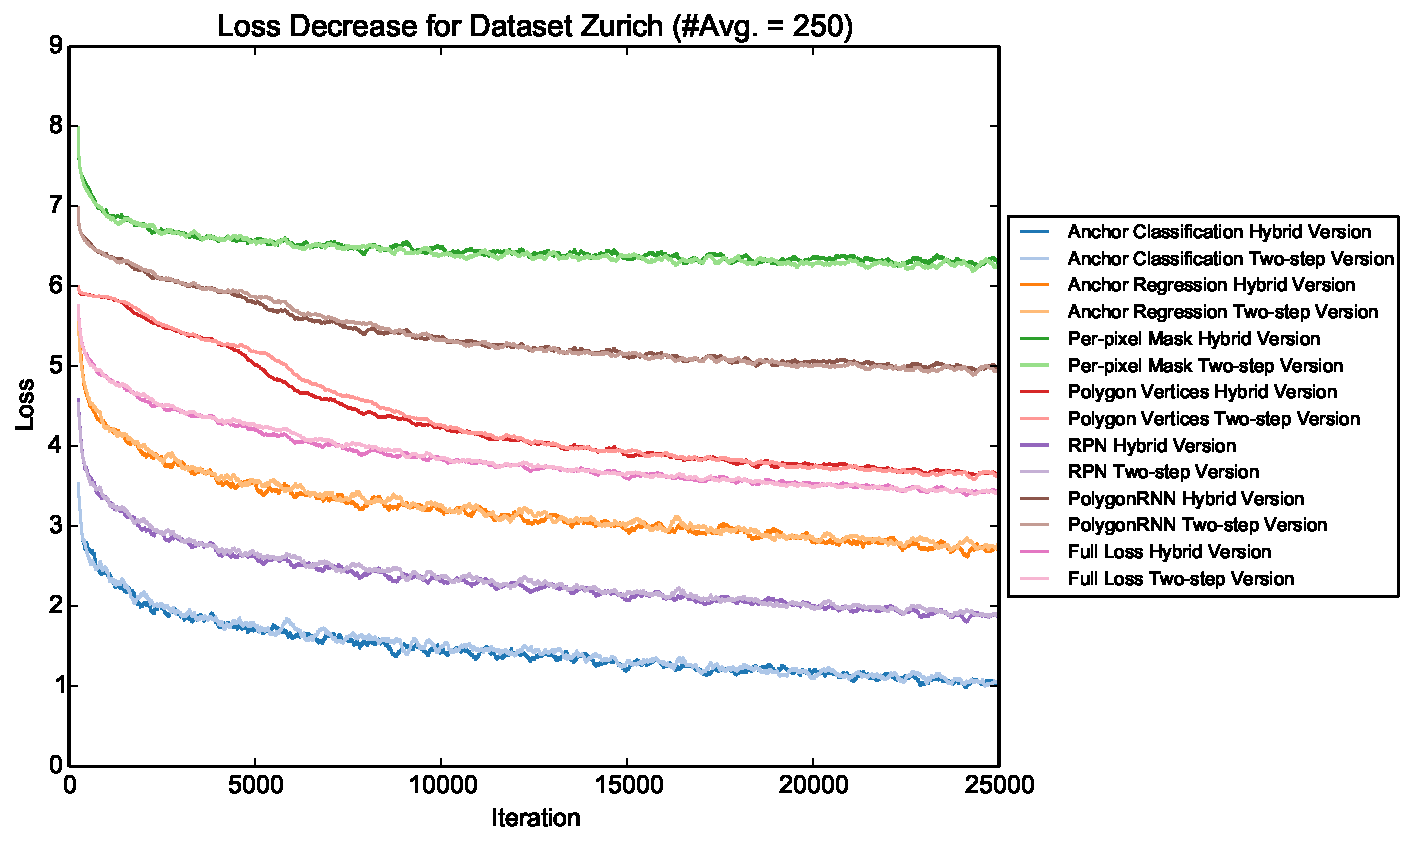
\includegraphics[width=\fig\textwidth]{4-07.pdf}
    \caption[Loss decrease of model in dataset Zurich]{Loss decrease of model in dataset Zurich.}
	\label{fig:losdeczh}
\end{figure}

In addition, we found that after completing 25,000 rounds on the training set of Zurich, the loss is still on the decline. However, because it has been trained for a long time and we want to compare it with Chicago under the same criterion, there is no further training for Zurich.

\subsection{Time Consumption}\label{tmcsmp}
We use the GPU resources from the Leonhard cluster of ETH Zurich to train our model and make prediction. The overall training time is around 48 hours for totally 25,000 rounds for a single model in the dataset of each city.

Table \ref{tab:timetrain} gives the time consumption for each batch of different models in different dataset when training. From the table we can conclude that the hybrid model has a negligible increase in training speed.
\begin{table}[!h]
	\centering
	\caption[Time spent by each batch in training phase]{Time spent by each batch in training phase.}
	\label{tab:timetrain}
	\begin{tabular}{l|r r}
	\hline
	\textbf{City} & Zurich & Chicago \\
	\hline
	\textbf{Two-step Version} & 7.237s & 7.150s \\
	\textbf{Hybrid Version} & 7.214s & 7.074s \\
	\hline
	\end{tabular}
\end{table}

Table \ref{tab:timepred} gives the time consumption of different models in different dataset when prediction. From the table we can conclude that no matter using what model or which dataset, they do not have obvious impact on the prediction time.
\begin{table}[!h]
	\centering
	\caption[Time spent in prediction phase]{Time spent in prediction phase.}
	\label{tab:timepred}
	\begin{tabular}{l|r|r|r|r|r}
	\hline
	\multicolumn{2}{l|}{\textbf{Stage}} & \multicolumn{2}{c|}{FPN} & \multicolumn{2}{c}{PolygonRNN\footnotemark[1]} \\ \hline
	\textbf{Model} & \textbf{BW\footnotemark[2]} & Chicago & Zurich & Chicago & Zurich \\ 	\hline
	\multirow{2}{*}{\begin{tabular}[c]{@{}l@{}}Two-step\\ Version\end{tabular}} & 6 & 1.414s & 1.421s  & 0.358s & 0.358s \\ 
	& 1 & 1.428s & 1.386s & 0.134s & 0.128s \\ \hline
\multirow{2}{*}{\begin{tabular}[c]{@{}l@{}}Hybrid\\ Version\end{tabular}} & 6 & 1.459s  & 1.458s & 0.358s & 0.360s \\ 
	& 1 & 1.451s  & 1.445s & 0.132s & 0.131s \\ \hline
\end{tabular}
\end{table}
\footnotetext[1]{Here the prediction time refers to the average time consumption of polygon extraction for a single building.}
\footnotetext[2]{BW refers to beam width.}

\subsection{Evaluation Metrics}\label{evalmtc}
Since the output of the model is an ordered sequence of pixel coordinates, it is difficult to find a suitable evaluation metric to quantize the degree of fitting between two polygons. Thus, the evaluation metrics we used are still traditional and pixel-based, of which we choose the weighted accuracy and F1 score. We also use IoU score, which can indicate the overlapping extent between two sets of pixels. The evaluation result with internal comparison can be seen in table \ref{tab:evalmodin}.

\begin{table}[!h]
	\centering
	\caption[Evaluation of models with internal comparison]{Evaluation of models with internal comparison.}
	\label{tab:evalmodin}
	\begin{tabular}{l|l|r|r|r|r}
	\hline
	\multirow{3}{*}{\textbf{Metric}} & \multirow{3}{*}{\textbf{City}} & \multicolumn{4}{c}{\textbf{Model}} \\ \cline{3-6}
	& & \multicolumn{2}{c|}{BW1\footnotemark[1]} & \multicolumn{2}{c}{BW6\footnotemark[1]} \\ \cline{3-6}
	& & Two-step & Hybrid & Two-step & Hybrid \\ \hline
	\multirow{2}{*}{Accuracy} & Chicago & 0.9043 & 0.8986 & \textbf{0.9105} & 0.9084 \\ \cline{2-6}
	& Zurich & 0.7856 & 0.8020 & 0.8129 & \textbf{0.8211} \\ \hline
	\multirow{2}{*}{F1 Score} & Chicago & 0.8672 & 0.8591 & \textbf{0.8777} & 0.8730 \\ \cline{2-6}
	& Zurich & 0.6711 & 0.7033 & 0.7171 & \textbf{0.7316} \\ \hline
	\multirow{2}{*}{IoU Score} & Chicago & 0.7922 & 0.7822 & \textbf{0.8037} & 0.7985 \\ \cline{2-6}
	& Zurich & 0.5486 & 0.5769 & 0.5937 & \textbf{0.6096} \\
	\hline
\end{tabular}
\end{table}
\footnotetext[1]{BW$x$ refers to beam width $x$.}

From table \ref{tab:evalmodin} we can see that the introduction of beam search improves the final result in all cases, especially for city Zurich using the IoU score evaluation. We also find that the two-step version does well on the dataset of Chicago, and the hybrid version does well on the dataset of Zurich. However, on the dataset of Chicago, two models have just slight difference, thus we still consider the hybrid version performs better. The evaluation result with external comparison can be seen in table \ref{tab:evalmodex}.

\begin{table}[!h]
	\centering
	\caption[Evaluation of models with external comparison]{Evaluation of models with external comparison.}
	\label{tab:evalmodex}
	\begin{tabular}{l|l|r|r|r|r}
	\hline
	\multirow{2}{*}{\textbf{Metric}} & \multirow{2}{*}{\textbf{City}} & \multicolumn{4}{c}{\textbf{Model}} \\ \cline{3-6}
	 & & Hybrid, BW6\footnotemark[1] & Paper \cite{polygonrnn} & Paper \cite{mspascal} & Thsis \cite{msnadine} \\ \hline
	\multirow{2}{*}{Accuracy} & Chicago & 0.9084 & \multirow{4}{*}{N/A} & \multirow{2}{*}{N/A} & \multirow{2}{*}{N/A} \\ \cline{2-3}
	& Zurich & 0.8211 & & \\ \cline{1-3}\cline{5-6}
	\multirow{2}{*}{F1 Score} & Chicago & \textbf{0.8730} & & 0.837 & 0.70 \\ \cline{2-3}\cline{5-6}
	& Zurich & 0.7316 & & \textbf{0.823} & \multirow{3}{*}{N/A} \\ \cline{1-5}
	\multirow{2}{*}{IoU Score} & Chicago & \textbf{0.7985} & \multirow{2}{*}{0.52--0.72\footnotemark[2]} & \multirow{2}{*}{N/A} & \\ \cline{2-3}
	& Zurich & 0.6096 & & & \\
	\hline
\end{tabular}
\end{table}
\footnotetext[2]{The IoU score here is for the cityscapes dataset (e.g. cars, trains, bicycles) in the original paper \cite{polygonrnn}, \textbf{NOT} for the dataset of aerial images of Zurich or Chicago.}

From table \ref{tab:evalmodex} we can see that our model outperforms the paper \cite{mspascal} and the thesis \cite{msnadine} with F1 score evaluation in the dataset of Chicago. As for the IoU evaluation, in the original paper of PolygonRNN, the IoU score typically falls into 0.52--0.72 for the cityscapes, thus our result of dataset Zurich is just normal. The reason why Chicago’s IoU score is relatively high is that most of the buildings are vertically or horizontally aligned.

\subsection{Prediction Results}\label{predres}
Figure \ref{fig:finalzh} and figure \ref{fig:finalch} presents the final prediction results on the test set of Zurich and Chicago respectively, using the hybrid version, beam width 6.

\begin{figure}[!h]
	\centering
	\includegraphics[width=\fig\textwidth]{4-08.png}
    \caption[Prediction results on the test set of Zurich]{Prediction results on the test set of Zurich. Note that multiple colors are used here to differentiate building instances.}
	\label{fig:finalzh}
\end{figure}
\begin{figure}[!h]
	\centering
	\includegraphics[width=\fig\textwidth]{4-09.png}
    \caption[Prediction results on the test set of Chicago]{Prediction results on the test set of Chicago. Note that multiple colors are used here to differentiate building instances.}
	\label{fig:finalch}
\end{figure}

(There will be more results here).
For more prediction results, please refer to section \ref{app:predzh} and \ref{app:predch}.


